\documentclass [MS] {uclathes}

%%%%%%%%%%%%%%%%%%%%%%%%%%%%%%%%%%%%%%%%%%%%%%%%%%%%%%%%%%%%%%%%%%%%%%%%
%                                                                      %
%                          PRELIMINARY PAGES                           %
%                                                                      %
%%%%%%%%%%%%%%%%%%%%%%%%%%%%%%%%%%%%%%%%%%%%%%%%%%%%%%%%%%%%%%%%%%%%%%%%

\title          {Augmenting MRI Classification with Synthetic Images \\
                Created via Generative Models}
\author         {Daniel Kwon}
\department     {Statistics}
\degreeyear     {2024}

%%%%%%%%%%%%%%%%%%%%%%%%%%%%%%%%%%%%%%%%%%%%%%%%%%%%%%%%%%%%%%%%%%%%%%%%

\chair          {Yingnian\ Wu}
\member         {...}
\member         {...}

%%%%%%%%%%%%%%%%%%%%%%%%%%%%%%%%%%%%%%%%%%%%%%%%%%%%%%%%%%%%%%%%%%%%%%%%

\abstract       {WIP - Check back later}

%%%%%%%%%%%%%%%%%%%%%%%%%%%%%%%%%%%%%%%%%%%%%%%%%%%%%%%%%%%%%%%%%%%%%%%%

\usepackage{subcaption} 
\usepackage{graphicx}
\usepackage{amsmath}
\usepackage{amsfonts}
\usepackage{array, makecell}
\usepackage{multirow}
\usepackage{float}
\usepackage{wrapfig,lipsum}
\renewcommand\cellset{\renewcommand\arraystretch{0.8}%
\setlength\extrarowheight{0pt}}

%%%%%%%%%%%%%%%%%%%%%%%%%%%%%%%%%%%%%%%%%%%%%%%%%%%%%%%%%%%%%%%%%%%%%%%%

\begin {document}

\makeintropages

%%%%%%%%%%%%%%%%%%%%%%%%%%%%%%%%%%%%%%%%%%%%%%%%%%%%%%%%%%%%%%%%%%%%%%%%

\chapter{Introduction}
With the performance of state-of-the-art generative models improving rapidly, synthetic images can be produced with ease 
using simple text or image prompts. Image generation models such as Dall-E or Stable Diffusion are able to create images 
with sufficient quality that the margin of difference between real and synthetic images is becoming increasingly thin. 
As the level of effort in generating synthetic images decreases and the quality of these images increases, the potential 
to use synthetic images as a means to augment image datasets becomes increasingly viable---especially in fields where 
gathering images is constrained by costs or other resources.

In the field of medical imaging, where image datasets often require specialized equipment and subject matter experts to 
capture and label images, gathering enough data to sufficiently train a classification model can be both expensive and 
time-consuming. For example, with the cost of magnetic resonance imaging (MRI) ranging from \$1,600 to \$8,400 in the 
United States, a dataset consisting of a few hundred images can exceed \$1 million; image classification models often 
require thousands of photos. 

One way computer vision models have historically attempted to remedy insufficient training datasets has been to employ 
traditional image augmentation techniques, which involve applying transformations such as flipping or blurring an 
original image to produce additional images for training. However, such transformations must be applied carefully in 
order to not lose the fidelity needed to make accurate diagnostic predictions. Transformations that alter the nature of 
the images can potentially lead to a degradation in model performance.

Augmenting image datasets with high quality synthetic images may allow for significant cost-saving while maintaining 
model performance, and previous research has found that synthetic images may play a complimentary role to image 
augmentation. The goal of this paper is to train image classification models on a MRI dataset to identify the presence 
of varying levels of dementia and investigate the effect of different image augmentation policies on model performance 
as well as compare their performance against an augmentation policy that generates synthetic images.

\chapter{Dataset}

\section{Alzheimer MRI Preprocessed Dataset}
For the purposes of this paper, we use publicly available MRI images of patients with varying levels of dementia, 
labeled as \textit{not demented}, \textit{very mildly demented}, \textit{mildly demented}, and \textit{moderately 
demented}. These images were downloaded via the datasets module provided and maintained by Hugging Face. All images are 
in black and white and have been pre-processed to 128x128 resolution.

\begin{figure}[H]
    \centering
    \subfloat[Not Demented]{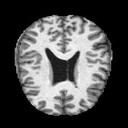
\includegraphics[width=0.225\textwidth]{figures/not-demented-example.png}\label{fig:f1}}
    \hfill
    \subfloat[Very Mildly Demented]{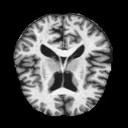
\includegraphics[width=0.225\textwidth]{figures/very-mild-demented-example.png}\label{fig:f2}}
    \hfill
    \subfloat[Mildly Demented]{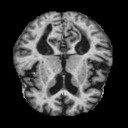
\includegraphics[width=0.225\textwidth]{figures/mild-demented-example.png}\label{fig:f3}}
    \hfill
    \subfloat[Moderately Demented]{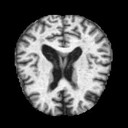
\includegraphics[width=0.225\textwidth]{figures/moderate-demented-example.png}\label{fig:f4}}
    \caption{Examples of real MRI images}
\end{figure}

\begin{table}[H]
    \centering
    \begin{tabular}{|>{\centering\arraybackslash}p{0.2\linewidth}|>{\centering\arraybackslash}p{0.2\linewidth}|>{\centering\arraybackslash}p{0.2\linewidth}|>{\centering\arraybackslash}p{0.2\linewidth}|} \hline 
        Not Demented & Very Mildly Demented & Mildly Demented & Moderately Demented\\ \hline 
        2566 & 1781 & 724 & 49\\ \hline
    \end{tabular}
    \caption{Count of each class in training data}
    \label{tab:my_label}
\end{table}

\section{Synthetic Images}
This paper utilizes OpenAI's Dall-E-2 to produce synthetic images. To generate synthetic images, an original image is 
supplied as a source and the generative models are prompted to creating a similar image.

In order to generate images using Dall-E-2 we utilize OpenAI's image variation API endpoint, which returns a variation 
of a given image. 

\begin{figure}[H]
    \centering
    \subfloat[Real Image]{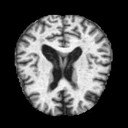
\includegraphics[width=0.25\textwidth]{figures/ModerateDemented_9.png}\label{fig:f1}}
    \hspace{0.1\textwidth}
    \subfloat[Synthetic Image]{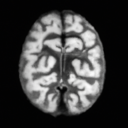
\includegraphics[width=0.25\textwidth]{figures/ModerateDemented_9_generated30.png}\label{fig:f2}}
    \caption{Results of Dall-E-2's image variation generation}
\end{figure}

Dall-E-2 reliably generates images that are similar to the real MRIs that are provided. Given that dementia is often 
physically tied to brain atrophy in certain areas, the synthetic images produced by Dall-E-2 generally reproduce the 
ridges, folds, and cavities of the source images as well.

\chapter{Exploration using Grad-CAM}
In order to better understand what parts of an image classification models deem to be more "important" in regards to 
predicting the presence of dementia, we employ Gradient-weighted Class Activation Mapping, or Grad-CAM, as a way to 
represent what a convolutional neural network "sees" when classifying both real and synthetic images. Grad-CAM is a 
technique that maps the gradients of a final convolutional layer in regards to a specific class prediction to product a 
heat map. The result is a visually intuitive way of illustrating which portions of an image contribute most to a given 
classification [source here].

\section{Overview of Grad-CAM}
\begin{enumerate}
    \item First, calculate the gradients of the model’s output in the final convolutional layer, with respect to the 
    feature maps. Assuming \(y_{c}\) is the score for class \(c\) (before softmax) and \(\delta A^{k}\) is the feature 
    map activation of the \(k\)th layer, compute \(\frac{\delta y_{c}}{\delta A^{k}}\). 
    
    \item Next, calculate the global average pooling of the feature map. Global average pooling is a pooling operation 
    designed to generate one feature map for each corresponding category of the classification task in the last 
    [convolutional] layer and then take the average of each feature map [source here].
    
    \[\alpha_{k}^{c} = \frac{1}{Z}\sum_{i}\sum_{j}\frac{\delta y_{c}}{\delta A_{ij}^{k}}\]

    \(Z\) here represents spatial dimensions of the feature map---in this case, its height and width. By dividing by 
    \(Z\), we obtain the average of gradients over all spatial locations. \(\frac{\delta y_{c}}{\delta A_{ij}^{k}}\) is 
    the gradient for class c with respect to the activation at \(A_{ij}^{k}\), or spatial location (i,j) on activation 
    layer \(k\).
    
    \item Lastly, we take the resulting importance weights in \(a_{k}^{c}\) and combine them with \(A^{k}\) to calculate 
    a weighted combination of all forward activation maps. We then apply the ReLU activation function to the resulting 
    combination in order to take the positive values only. This ensures that we are only looking parts of the image that 
    are positively correlated with a given class.

    \[L_{Grad-CAM}^{c} = ReLU(\sum_{k}\alpha_{k}^{c}A^{k})\]

    Notice that \(L_{Grad-CAM}^{c}\) will have the dimensions of the final convolutional layer and therefore is likely 
    to be smaller than the original input image. In that case, we simply upsample the result to the dimensions of our 
    original image in order to overlay the two.
\end{enumerate}

\section{Exploratory Results}
WIP

\chapter{Background on Training Deep Learning Models}

\section{Overview of Neural Networks}
While deep learning architectures can span many layers and can incorporate many different mechanisms, at its core all 
deep learning models are neural networks. Training neural networks comprise of a few key steps. 

First, training data is input into a neural network and passed through as-is in what is known as a "forward pass." In a 
fully connected neural network, every individual neuron in a layer of the neural network is connected to each neuron in 
the preceding layer 

\begin{figure}[H]
    \centering
    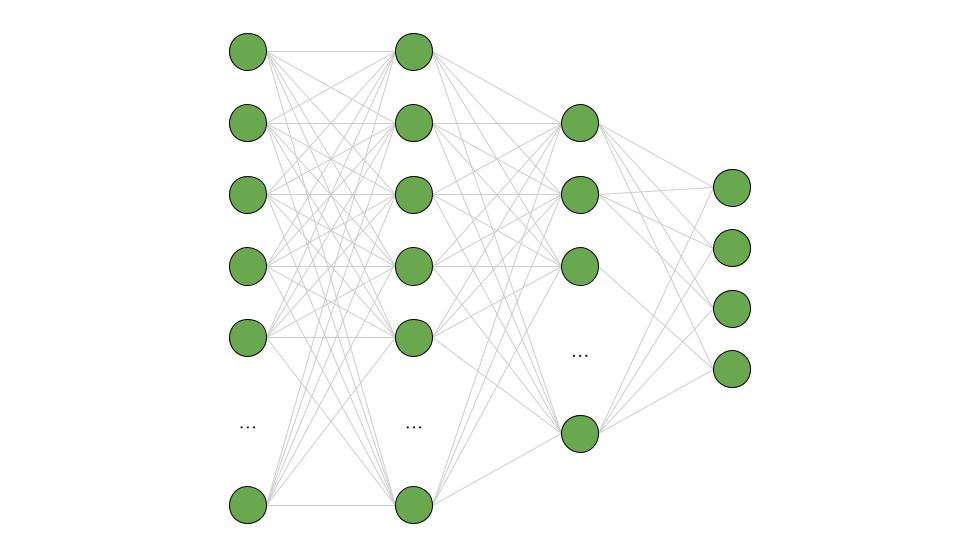
\includegraphics[width=0.75\linewidth]{figures/NN_diagram.jpg}
    \caption{An illustration of a  typical fully-connected neural network}
    \label{fig:enter-label}
\end{figure}

Each of these connections has a weight that stores how strong of a connection each preceding node has to the current 
node. A bias term is also present, which represents whether a neuron is general activated or not. Often, an initialized 
neural network will comprise of randomized weights and biases whereas a pre-trained model will have the weights and 
biases already defined from previous training. When training a neural network, the weights and biases are what are being 
adjusted in order to minimize loss. The formulation of a single neuron with n nodes in the previous layer is below:

\[\sigma(w_0a_0 + w_0a_0 + w_0a_0 + ... + + w_{n-1}a_{n-1} + b)\]

After the forward pass, backpropagation occurs in which the gradient (the vector of partial derivatives) of the loss 
function with respect to each weight and bias is calculated via chain rule. Each gradient value represents the magnitude 
and direction of the change in our loss function given a change to that particular weight or bias. Because 
backpropagation uses the chain rule to propagate the loss backward from the output layer to the input layer, the process 
of finding the gradient of a loss function remains the same no matter how many layers are in the network or how many 
neurons are in each layer.

Once the gradient is calculated, the gradient descent algorithm is used to update the weights and biases in order to 
minimize loss. However, applying the gradient descent on an entire training dataset in a single batch is computationally 
expensive. Instead, gradient descent is often applied to subsets of the training data, called mini-batches. Each 
training iteration, or epoch, will then take a mini-batch to apply the forward and backward passes on to to updates its 
weights and biases. The result is an accurate approximation of the gradient of the loss function while significantly 
decreasing computational expenses [source].

\section{Loss Function}
The loss function used throughout this paper when measuring model performance is cross entropy loss. Cross entropy loss 
is defined as:

\[L = -\sum_{c=1}^{C}y_{c}log(p_{c})\]

where \(C\) = the number of classes, \(y_{c}\) is the true label for class, and \(p_{c}\) is the predicted probability 
for class \(c\). Cross entropy loss therefore compares the predicted probabilities with the actual labels and penalizes 
more when the predicted probabilities for a correct class is low [source].

Cross entropy loss is better suited for measuring the performance of classification models when multiple classes are 
involved than traditional measures of error, such as the sum of residuals, as it is more sensitive to predictions that 
are "more" incorrect. In an image classification problem, a model may mislabel a given image, but the cross entropy loss 
will be lower if the predicted probability for the correct class is higher, even if the model did not ultimately end up 
labeling correctly. Contrast that with the sum of residuals, which only views predictions as completely correct or 
completely incorrect and fails distinguish between the degrees of how right or wrong a prediction can be [source].

\begin{figure}[H]
    \centering
    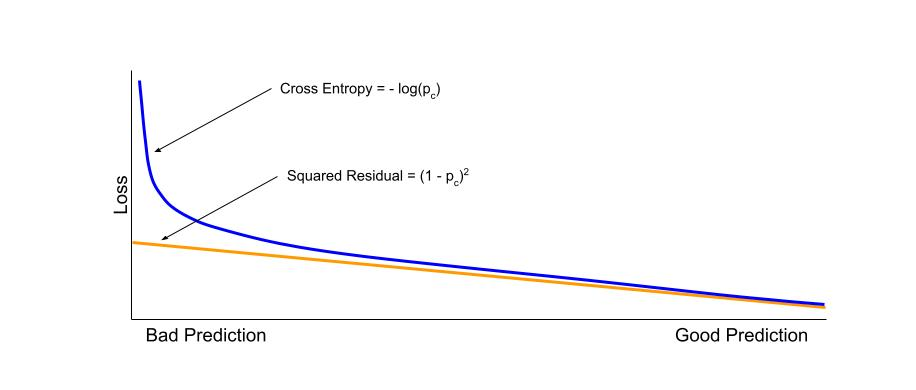
\includegraphics[width=1\linewidth]{figures/CE vs Square Residual.jpg}
    \caption{Illustration of Cross Entropy Loss vs Squared Residual}
    \label{fig:enter-label}
\end{figure}

Take for example, when the true label is 1 and the predicted class weight \(y_{c}\) is 0.0001---making our model 
prediction very bad. The squared residual would be \((1-0.0001)^{2} = 0.9998\) while our cross entropy loss would be 
more punitive at \(-log(0.0001) = 4\). Cross entropy loss also has a much larger gradient for very bad predictions, 
allowing our model to more quickly learn to avoid bad predictions.

\section{Gradient Descent}
As mentioned previously, performing gradient descent on every single training image can be computationally inefficient. 
Instead, stochastic gradient descent which divides the training dataset into smaller batches and applied the gradient 
descent algorithm on each batch, can significantly reduce runtime. 

In addition to dividing the training dataset into mini-batches, there are other methods that make optimization via 
gradient descent more efficient---namely, learning rate and momentum.

\subsection{Learning Rate}
The formulation for stochastic gradient descent is defined as:
\[\theta_{t+1} = \theta_{t} - \eta\nabla_{\theta}L(\theta_{t};x^{(i)})\]
Where:
\begin{itemize}
    \item \(\theta_{t}\) is the model's weights and biases at iteration \(t\)
    \item \(\eta\) is the learning rate
    \item \(\nabla_{\theta}L(\theta_{t};X^{(i)})\) is the gradient of the loss function at time \(t\) with respect to 
    \(x^{(i)}\)
    \item \(x^{(i)}\) is a randomly selected mini-batch
\end{itemize}

The learning rate is a critical parameter for the training of any deep learning model and can dramatically effect how 
the gradient descent algorithm behaves. Learning rate can be understood intuitively as the step size the optimization 
algorithm takes when it decides which direction to step---too large of a learning rate can lead to sub-optimal changes 
to a network's weights and biases; too small and achieving model convergence can much longer.

Furthermore, the learning rate does not necessarily need to be constant throughout the entire optimization process. It 
can vary over time with a larger learning rate at the beginning of the training, when large steps along the gradient is 
appropriate, and reducing later in training process, when smaller learning rates are more appropriate.

\subsection{Momentum}
Momentum takes into account the gradient at previous steps, beyond simply looking at the gradient at time \(t-1\). By 
doing so, the gradient descent algorithm tends to stay in the direction where the gradient has consistently pointed 
towards. The formulation for stochastic gradient descent with momentum is defines as:
\[\theta_{t+1} = \theta_{t} - \eta v_{t}\]
Where \(v_{t}\) is known as the velocity term, defined as:
\[v_{t} = \beta v_{t-1} + (1 - \beta) \nabla_{\theta} L(\theta_{t})\]
Where:
\begin{itemize}
    \item \(\beta\) is the momentum coefficient, which determines how much of the previous gradients carry over into the 
    latest velocity calculation at time \(t\)---this parameter can be set between 0 and 1
    \item \(\nabla_{\theta} L(\theta_{t})\) is the gradient of the loss function at time \(t-1\)
\end{itemize}

\subsection{Adam Optimizer}
Adaptive Moment Estimation, also known as Adam Optimization, combines aspects of both a variable learning rate as well 
as momentum in order to develop an optimization algorithm that efficiently calculates the gradient. Gradient descent 
using Adam optimization is defined as:
\[\theta_{t+1} = \theta_{t} - \frac{\eta}{\sqrt{\hat{v_t}} + \epsilon} \hat{m_{t}}\]
Where:
\begin{itemize}
    \item \(\hat{m_{t}}\) is known as the bias correction for the first moment and defined as \(\frac{m_t}{1-\beta_1^t}\)
    \item \(\hat{v_t}\) is known as the bias correction for the second momemt and defined as \(\frac{v_t}{1-\beta_2^t}\)
    \item \(m_t = \beta_1 m_{t-1} + (1 - \beta_1) \nabla_{\theta} L(\theta_t)\)
    \item \(v_t = \beta_2 v_{t-1} + (1 - \beta_2) (\nabla_{\theta} L(\theta_t))^2\)
    \item \(\beta_1\) is the decay rate for the first moment
    \item \(\beta_2\) is the decay rate for the second moment
\end{itemize}

The first moment \(m_t\) allows the Adam optimization algorithms to take into account momentum by taking the weighted 
average of past gradients. The second moment \(v_t\) acts as an adjustment to the learning rate and allows Adam 
algorithm to have a variable learning rate based on previous squared gradients. For all models trained in this paper, we 
use the Adam optimizer.

\subsection{Fine-tuning Pre-trained Models}
Often times, computer vision models require a large number of images as well as a significant amount of computation 
time. In order to accelerate the training process, many image classification models will utilize a pre-trained model, 
instead of starting training from randomly initialized weights and biases. The most common image dataset used to 
pretrain models is the ImageNet-1000 dataset, which is comprised of 1000 distinct classes, 1,281,167 training images, 
50,000 validation images and 100,000 test images.

Once a model is pre-trained, fine-tuning can take two forms---either progressing through training as you normally would
with images intended for fine-tuning (i.e., your dataset) or freezing all weights in the pre-trained model (essentially 
locking the model from any further training) and re-training only the fully connected neural nerwork appended to the 
pre-trained model. If the latter method is used, the pre-trained model can regarded as a fixed feature extractor for an 
image. For the purposes of our paper, all pre-trained models are fine-tuned by re-training on our dataset.

\chapter{Overview of Model Architectures}
In order to gain an understanding as to how both convolution-based and attention-based architectures react to the 
introduction to synthetic data in training, We tested three different deep learning model architectures for our image 
classification models---a basic Convolutional Neural Network (CNN), a pretrained ResNet-18 model, and a pretrained 
Vision Transformer (ViT).

\section{Convolutional Neural Networks}

\begin{figure}[h]
    \centering
    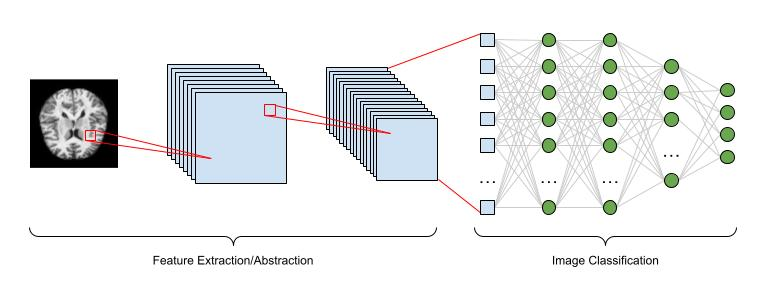
\includegraphics[width=0.9\linewidth]{figures/CNN-diagram.jpg}
    \caption{Typical CNN Architecture}
    \label{fig:synthetic-mix}
\end{figure}

CNNs are a deep learning architecture that is comprised of convolutional layers---which abstract an image to a feature 
map, pooling layers---which reduce the dimensions of data by combining the outputs of adjacent layers via downsampling, 
and fully connected layers---which are neural networks that take the final activations from the convolutional and 
pooling layers to generate class weights.

Convolutional layers are a key component of convolutional neural networks and act as a way for the network to 
extract abstract features from an image. The primary operating mechanism of a convolutional layer comprises of a kernel,
or a filter that is applied to the original image.

\begin{figure}[H]
    \centering
    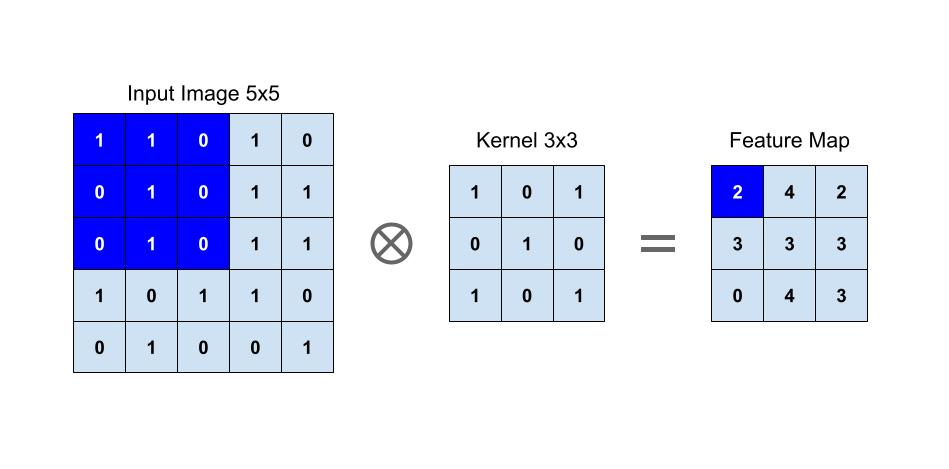
\includegraphics[width=0.6\linewidth]{figures/convolutional_layer_illustration.jpg}
    \caption{Illustration of Convolutional Layer}
    \label{fig:synthetic-mix}
\end{figure}

Often, convolutional layers may stack multiple kernels resulting in activation maps with more channels. As subsequent 
layers get deeper, more complex and increasingly abstract features are extracted from the original image. While the 
kernels from the earlier layers of a CNN may learn to identify basic shapes and patterns, kernels in deeper layers may 
learn to identify specific edges and details.

\begin{figure}[H]
    \centering
    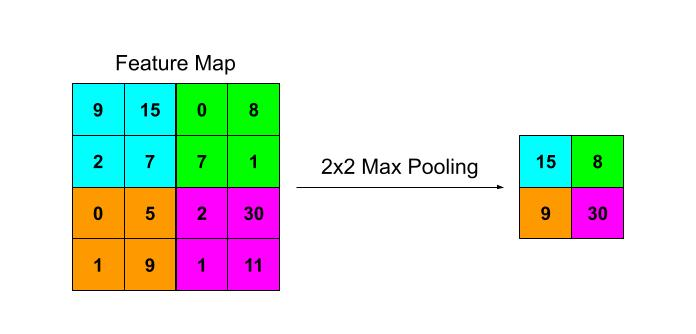
\includegraphics[width=0.55\linewidth]{figures/maxpooling_illustration.jpg}
    \caption{Illustration of 2x2 Max Pooling}
    \label{fig:maxpooling-illust}
\end{figure}

Though not explicitly required, max pooling layers frequently follow convolutional layers. Max pooling layers 
essentially downsample the activation map so that the important features and spatial relationships contained in an image
are captured while removing unnecessary details and reducing the feature map's dimensions, thereby improving 
computational efficiency of the network.

\begin{figure}[H]
    \centering
    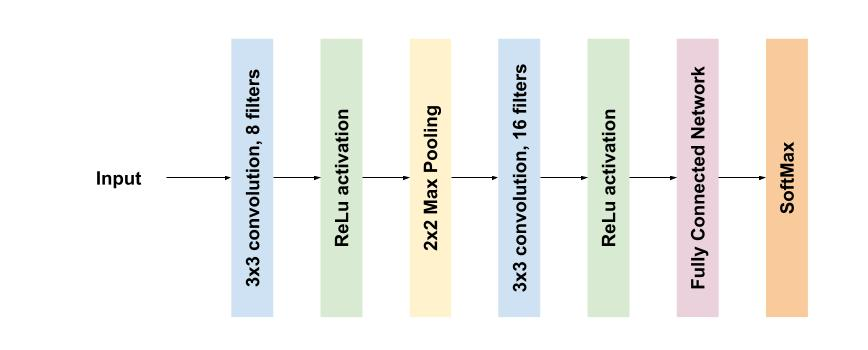
\includegraphics[width=0.8\linewidth]{figures/basic_cnn_architecture.jpg}
    \caption{Basic CNN Architecture}
    \label{fig:cnn-architecture}
\end{figure}

For the purposes of this paper, the CNN we train from scratch consists of 2 convolutional layers, each paired with a 
ReLU activation function and a max pooling layer. After all feature extraction layers are complete, the final activation 
layer is fed into a fully connected neural network with 2 hidden layers and an output layer that predicts probabilities 
weights for each of our four classes.

\section{ResNet-18}
The second model architecture we test is a ResNet-18 model, pre-trained on the ImageNet-1000 dataset. The ResNet 
architecture is similar to a basic convolutional neural network but adds two additional components---skip connections 
and residual blocks.

\begin{figure}[H]
    \centering
    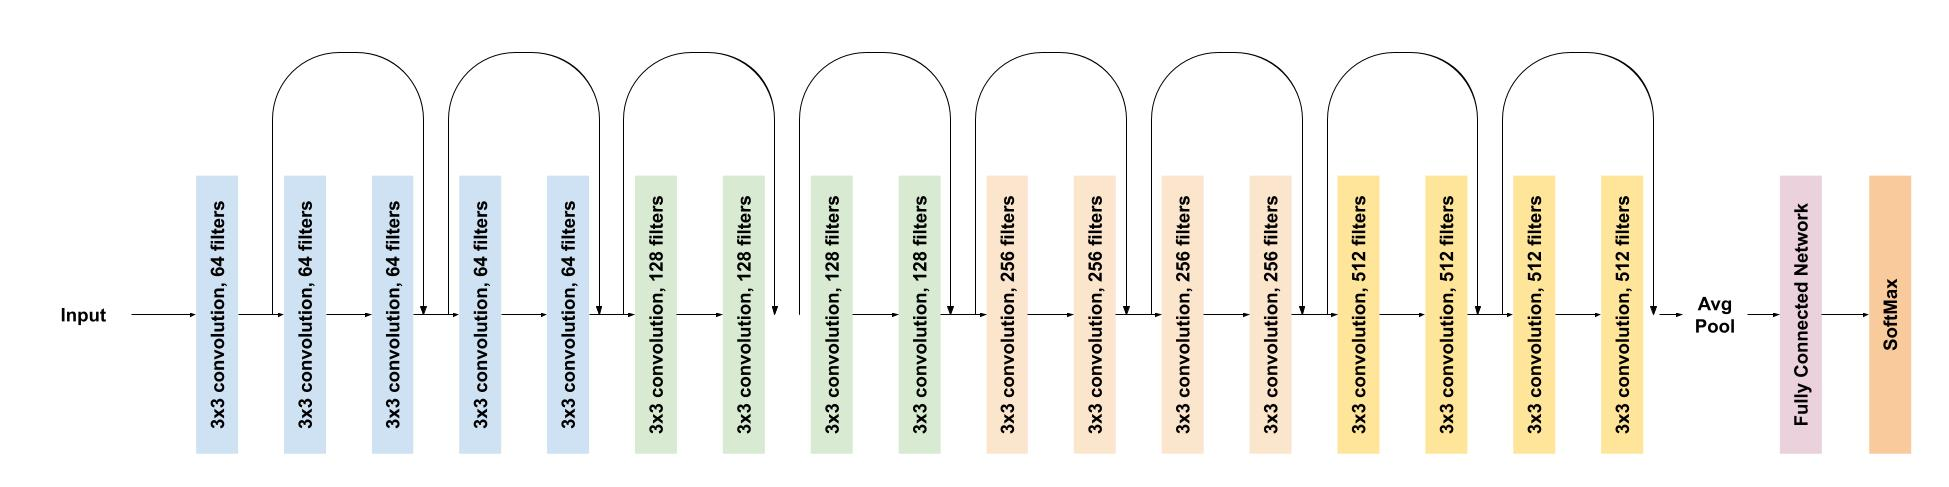
\includegraphics[width=1\linewidth]{figures/resnet18_architecture.jpg}
    \caption{ResNet-18 Architecture}
    \label{fig:resnet-architecture}
\end{figure}

Skip connections allow the network to skip a convolutional layer entirely thereby skipping training for some layers.
Doing so helps to avoid a phenomenon known as vanishing gradients---which occurs in deep networks where the gradient 
calculated via backpropagation becomes so small that weights from earlier layers become insignificant and changes to the 
input image cease to meaningfully affect feature mapping in deeper layers. Skip connections allow the ResNet model to 
build deep networks while avoiding vanishing gradients by giving the model a mechanism in which training a layer can be 
skipped entirely.

ResNet architectures are also characterized by their use of residual blocks, which consistent of 2 convolutional layers 
and a skip connection. Residual blocks allow the ResNet model to train on the residual between layers, or the difference 
between the input and the ideal output of the layers. 

\[y = F(x) + x\]

Where:
\begin{itemize}
    \item \(x\) is input fed into the residual block
    \item \(F(x)\) is output coming from the residual block
    \item \(y\) is desired final output coming from the residual block
\end{itemize}

Therefore, \(F(x) = y - x\) makes \(F(x)\) the residual of y and x. ResNets train by using residual blocks to learn the 
residual mapping, instead of being forced to train each convolutional layer and the desired feature map (although that 
is still an option left for the model to evaluate). By doing so, the ResNet remains computationally efficient while 
maintaining the ability to extract features, either through its traditional convolutional layers or via a residual 
block. 

\section{Vision Transformers}
The last type of model architecture tested is one that foregoes the use of convolutional layers entirely. Instead, 
vision transformers utilize the attention mechanism to capture spatial relationships and abstract features.

\chapter{Methodology}
\section{Traditional Image Augmentation Policies}
\section{Synthetic Image Generation Policy}
Given a desired proportion of original training images to utilize (\textit{X}) and the desired proportion of synthetic 
images to augment the training data (\textit{Y}), we combine both synthetic and original images to train our image 
classification model. 

\begin{figure} [h]
    \centering
    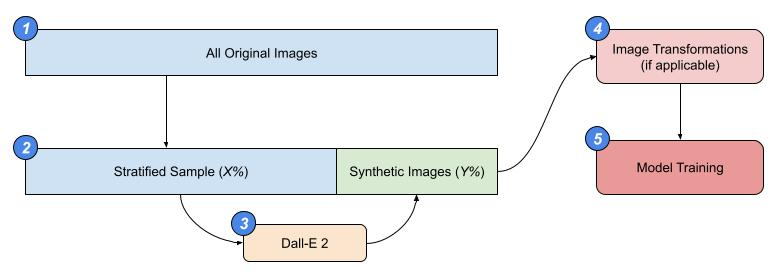
\includegraphics[width=1\linewidth]{figures/image_generation_policy.jpg}
    \caption{Enter Caption}
    \label{fig:enter-label}
\end{figure}

The figure above illustrates one iteration of our image generation policy in order to generate our mixed training set 
(i.e., containing both original and synthetic images)
\begin{enumerate}
    \item First, we take a random stratified sample of our original images
    \item The stratified sample is sent to Dall-E 2 via OpenAI's API in order to generate an image variation
    \item Image transformations are applied to our entire mixed training set (if applicable)
    \item Mixed training set, post transformations/augmentation, is used to train the image classification model
    \item Steps 1-4 are repeated \textit{N} times in order to account for the stochastic nature of Dall-E's responses as 
    well as to bootstrap a distribution of performance--measured by cross entropy loss
\end{enumerate}


\chapter{Results}

\section{CNN Results}
When applied to a basic convolutional neural network, augmentation via synthetic images provides the most benefit when 
the dataset of original images is limited. When training our CNN on a 30\% stratified sample, the median validation loss 
from 100 simulations was 0.219863, compared to a loss of 0.176023 when training on the full dataset---resulting in an 
increase in our loss by approximately 25\%.

However, model performance improves when augmenting the 30\% stratified training sample with synthetic images so that 
the resulting training set contains the same number of images as the full training data set. The resulting model trained 
on the mix of 30\% real and 70\% synthetic images has a cross-entropy loss of 0.174202---a decrease of over 20\% 
compared to the model trained on only the 30\% of real training images and matching the performance of model trained on 
the entirety of the training images.

\begin{figure}[H]
    \centering
    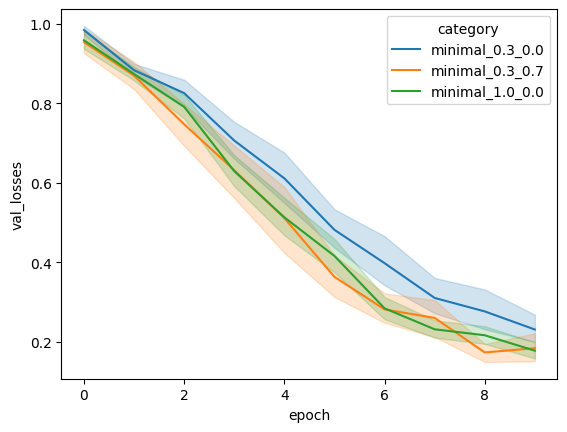
\includegraphics[width=0.7\linewidth]{figures/cnn_minimal30_result.png}
    \caption{Cross Entropy Loss - Model trained on 30\% Real, 70\% synthetic}
    \label{fig:enter-label}
\end{figure}

Moreover, CNNs trained on synthetic data outperformed CNNs trained on 30\% of available training images and paired with 
traditional image augmentation policies. This is likely due to the fact that the image augmentation policies may alter 
the nature of the image enough to degrade performance of our classification model. This is not to say that traditional 
image augmentation methods do not have a role in medical imaging; only that traditional image segmentation policies, 
when misapplied, can degrade model performance significantly and therefore likely require subject matter experts to 
evaluate whether image augmentation is necessary. In fact, other studies have found that image augmentation generally 
improves the performance of image classification models used for brain imaging. 

\begin{figure}[H]
    \centering
    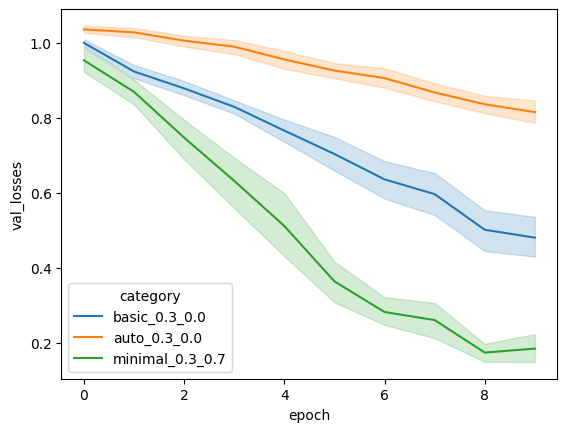
\includegraphics[width=0.7\linewidth]{figures/image_augmentation_comparison.png}
    \caption{Comparison of resulting cross entropy loss across models using different image augmentation policies, all 
    trained on 30\% of available images}
    \label{fig:enter-label}
\end{figure}
However, not all training datasets benefit from synthetic image augmentation. CNNs trained on 40-80\% of all available 
training data resulted in virtually no improvement, with the 80\% model resulting in a degradation in loss. This alludes 
to the possibility that synthetic data augmentation may be more beneficial as original training data becomes more 
constrained.

\chapter{Conclusion}

\chapter{Additional Considerations}

\end {document}